% !TeX spellcheck = en_US
\addsection{All Map Locations}{\skills/earth_magic.png}

\begin{multicols*}{2}

\hypertarget{All}{This} section describes the function of Fields not explained above.
The following \textbf{Visitable} fields are not pictured out of redundancy, as their effects are described clearly by the symbols on the right:
\begin{itemize}
  \item Artifact Symbol
  \item Fountain of Youth
  \item Learning Stone
  \item Mystical Garden
  \item Pandora's Box
  \item Resource Symbol
  \item Shrine of Magic Gesture/Incantation
  \item Temple
  \item Treasure Symbol
  \item Warrior's Tomb
  \item Water Wheel
  \item Windmill
\end{itemize}

\vspace*{\fill}
  \vspace{4.4em}
\note{10}{
  The effects of Fields that allow you to \textbf{Search} for Spells or Artifacts, or where you must spend resources to use the Field's effect, are \textbf{always optional}.
  You must always place a Black Cube on such Visitable Fields even if you choose not to use that Field's effect.
}
\vspace*{\fill}
\columnbreak

\begin{center}
  \framedimage[\linewidth]{\tables/symbols.png}
\end{center}

\pagebreak

\subsection*{Towns, Mines and Settlements}
\textbf{Towns} are always located in the center of a Starting (I) Tile.
Flagging an enemy Town prevents their Secondary Heroes from spawning there and Main Heroes from moving there if defeated.
Flagging a Town can cause \hyperlink{End}{Player Elimination}, and Scenarios typically have special rewards for Flagging them.
Flagging a Town also gives you a \textbf{Faction Cube} from its original owner.
Otherwise, Flagging a Town does not affect its original owner in any way.
They do not lose access to their Town board or its functions.
You also do not gain access to their Town board or Faction Units, unlike in the video game.

\begin{center}
  \framedimage[\linewidth]{\images/core_towns.jpg}
  \textit{Towns from the core game.}
\end{center}

\medskip

\hypertarget{Mines}{\textbf{Mines}}\index{Mines} are Flaggable Fields which increase a specific resource's income when Flagged.
If you are the first one to Flag a mine, it also immediately provides you with its income.
All mines have the \includesvg[height=10px]{\svgs/ongoing.svg} symbol and a picture of the Resource they produce next to it.

\begin{center}
  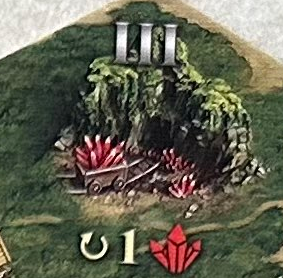
\includegraphics[width=0.6\linewidth]{\images/mine_example.png}\\
  \textit{A mine that produces \includesvg[height=10px]{\svgs/valuablegreater.svg}, guarded by Level 3 Neutral Units.
    The first player to Flag this Field would immediately gain one \includesvg[height=10px]{\svgs/valuablegreater.svg} in addition to increasing their \includesvg[height=10px]{\svgs/valuablegreater.svg} income.
  }
\end{center}
\columnbreak

\textbf{Settlements}\index{Settlement} act as a spawn point for Secondary Heroes, and as a place for Main Heroes to move to when defeated.
When you Flag a Settlement, choose whether to increase your \includesvg[height=10px]{\svgs/gold.svg}, \includesvg[height=10px]{\svgs/building_materials.svg} or \includesvg[height=10px]{\svgs/valuablegreater.svg} income by one space.
As with Mines, if you are the first player to Flag a Settlement, you immediately gain Resources equal to that increase in production.
Mark the Settlement with an appropriate Resource Token to show which Resource it produces.
When you Flag an enemy Settlement, you may change which Resource it produces.\par
Additionally, \textbf{instead of increasing Resource Production}, you may choose to \textbf{Reinforce} one of your \includesvg[height=10px]{\svgs/bronze.svg} or \includesvg[height=10px]{\svgs/silver.svg} Units immediately for half the normal cost, rounded up.
If you were the first player to Flag the Settlement, Reinforce that Unit \textbf{for free} instead.
Do not place any Resource Tokens on the Settlement if you choose to Reinforce.

\bigbreak

\begin{minipage}[h]{\linewidth}
  \centering
  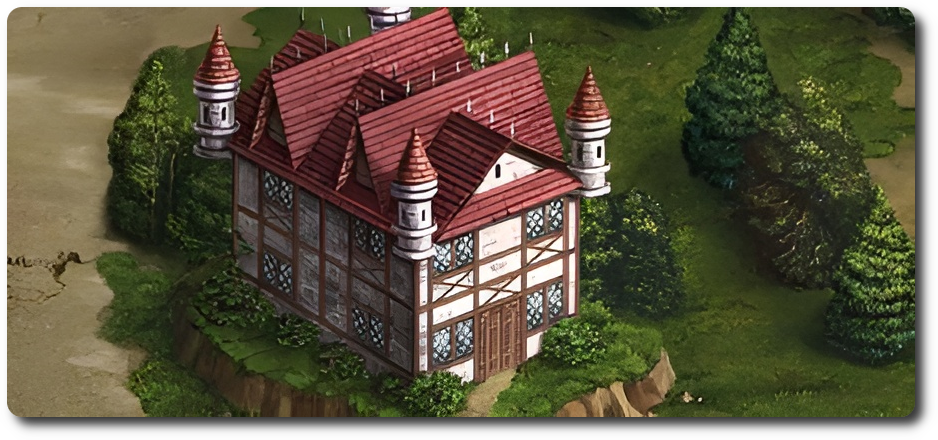
\includegraphics[width=0.44\linewidth]{\map_locations/castle_settlement.png}
  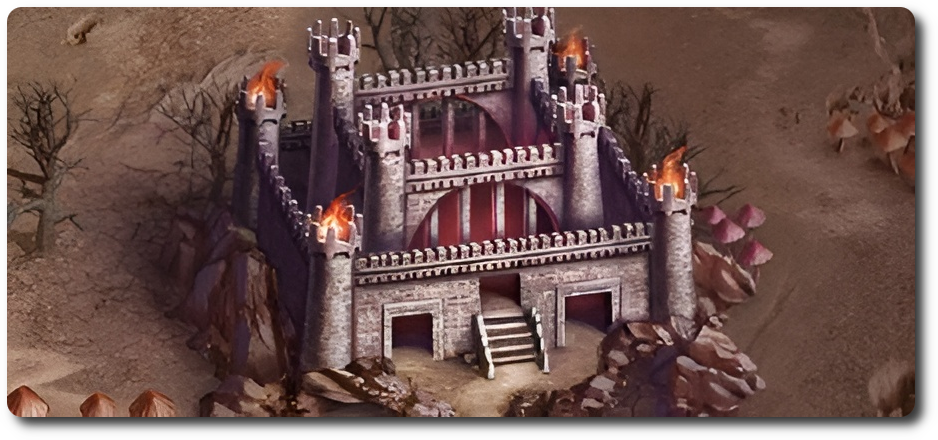
\includegraphics[width=0.44\linewidth]{\map_locations/dungeon_settlement.png}
  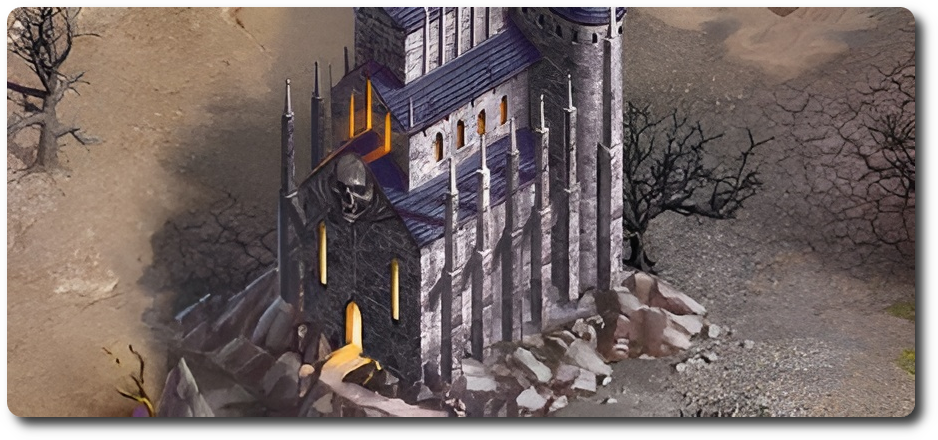
\includegraphics[width=0.44\linewidth]{\map_locations/necropolis_settlement.png}
  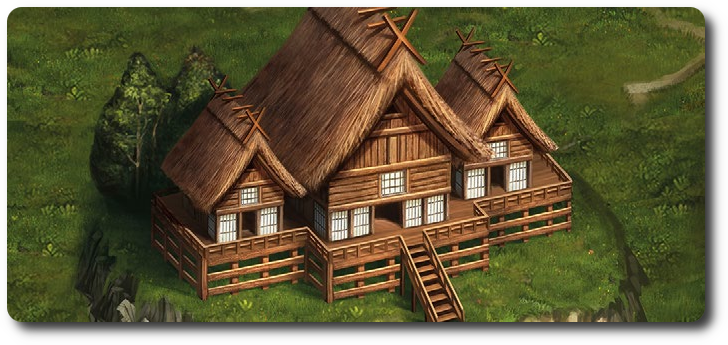
\includegraphics[width=0.44\linewidth]{\map_locations/rampart_settlement.png}
  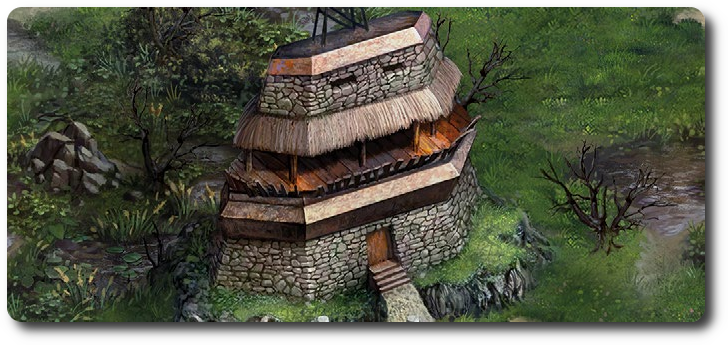
\includegraphics[width=0.44\linewidth]{\map_locations/fortress_settlement.png}
  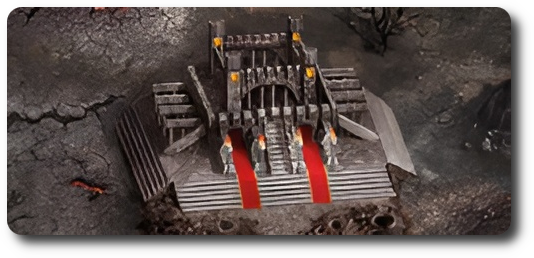
\includegraphics[width=0.44\linewidth]{\map_locations/inferno_settlement.png}
  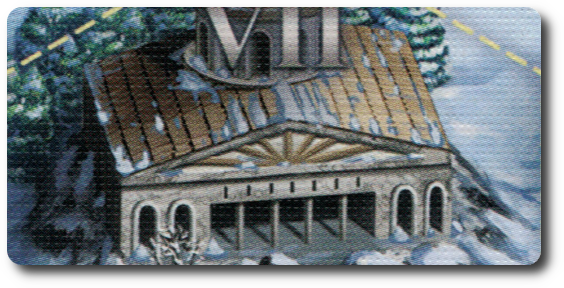
\includegraphics[width=0.4\linewidth]{\map_locations/tower_settlement.png}
  \par
  \textit{All possible Settlements.
  Each is styled after a different Faction.
  They all work identically.}
\end{minipage}
\end{multicols*}
\bigbreak

\subsection*{Revisitable Fields}

\begin{figure}[H]
  \begin{minipage}[t]{0.47\textwidth}
    \vspace{0pt}
    \centering
    \textbf{Library}\par
    \framedimage[\textwidth]{\map_locations/library.jpg}
    \caption{\small Category: \textbf{Revisitable}\\You may
      \includesvg[height=8px]{\svgs/pay_v2.svg}
      3 \includesvg[height=8px]{\svgs/gold.svg}
      to Remove 1 Statistic Card from your hand or Discard Pile and replace it with any other Statistic Card.
      You may do this twice per Visit.}
  \end{minipage}\hfill
  \begin{minipage}[t]{0.47\textwidth}
    \vspace{0pt}
    \centering
    \captionsetup{singlelinecheck=off}
    \phantom{j}\textbf{Black Market}\par
    \framedimage[\textwidth]{\map_locations/black_market.jpg}
    \caption[black market]{\small Category: \textbf{Revisitable}\\Look at the top 4 cards from the Artifact Discard Pile.
      You may buy one of them for:
      \begin{itemize}
      \setlength\itemsep{-4pt}
        \item [5] \includesvg[height=8px]{\svgs/gold.svg} if it is a \textbf{Minor} Artifact
        \item [7] \includesvg[height=8px]{\svgs/gold.svg} if it is a \textbf{Major} Artifact
        \item [10] \includesvg[height=8px]{\svgs/gold.svg} if it is a \textbf{Relic} Artifact
      \end{itemize}
      }
  \end{minipage}
\end{figure}

\begin{figure}[H]
  \begin{minipage}[t]{0.47\textwidth}
    \vspace{0pt}
    \centering
    \textbf{Sanctuary}\par
    \framedimage[\textwidth]{\map_locations/sanctuary.jpg}
    \caption{\small Category: \textbf{Revisitable}\\
      Heroes on this Field cannot be attacked by other Heroes.
      Friendly Heroes can move through enemy Heroes on this Field but cannot stop here.}
  \end{minipage}\hfill
  \begin{minipage}[t]{0.47\textwidth}
    \vspace{0pt}
    \centering
    \phantom{j}\textbf{Tavern}\par
    \framedimage[\textwidth]{\map_locations/tavern.jpg}
    \caption{\small Category: \textbf{Revisitable}\\
      You can \includesvg[height=8px]{\svgs/pay_v2.svg}
      7 \includesvg[height=8px]{\svgs/gold.svg}
      to gain a Secondary Hero.
      Place their model on this Field.
      Then, choose one enemy player to discard 1 random card from their hand.}
  \end{minipage}
\end{figure}

\begin{figure}[H]
  \begin{minipage}[t]{0.47\textwidth}
    \vspace{0pt}
    \centering
    \hypertarget{Trading Post}{\textbf{Trading Post}}\par
    \framedimage[\textwidth]{\map_locations/trading_post.jpg}
    \caption{\small Category: \textbf{Revisitable}\\
      \textbf{Choose one}: \protect\hyperlink{Trading}{Trade} resources and Remove cards OR buy a \protect\hyperlink{War Machines}{War Machine}.
    }
  \end{minipage}\hfill
  \begin{minipage}[t]{0.47\textwidth}
    \vspace{0pt}
    \centering
    \phantom{j}\hypertarget{War Machine Factory}{\textbf{War Machine Factory}}\par
    \framedimage[\textwidth]{\map_locations/war_machine_factory.jpg}
    \caption{\small Category: \textbf{Revisitable}\\Buy a \protect\hyperlink{War Machines}{War Machine}.\phantom{.......}}
  \end{minipage}
\end{figure}

\begin{figure}[H]
  \begin{minipage}[t]{0.47\textwidth}
    \vspace{0pt}
    \centering
    \phantom{j}\textbf{Stables}\par
    \framedimage[\textwidth]{\map_locations/stables.jpg}
    \caption{\small Category: \textbf{Revisitable}\\
      Gain 1 MP \includesvg[height=8px]{\svgs/movement.svg}.
      It lasts for only one Turn.
      See \protect\hyperlink{Movement}{Movement Actions}.
    }
  \end{minipage}\hfill
\end{figure}

\begin{tikzpicture}[overlay]
  \node at (16, 4.5) {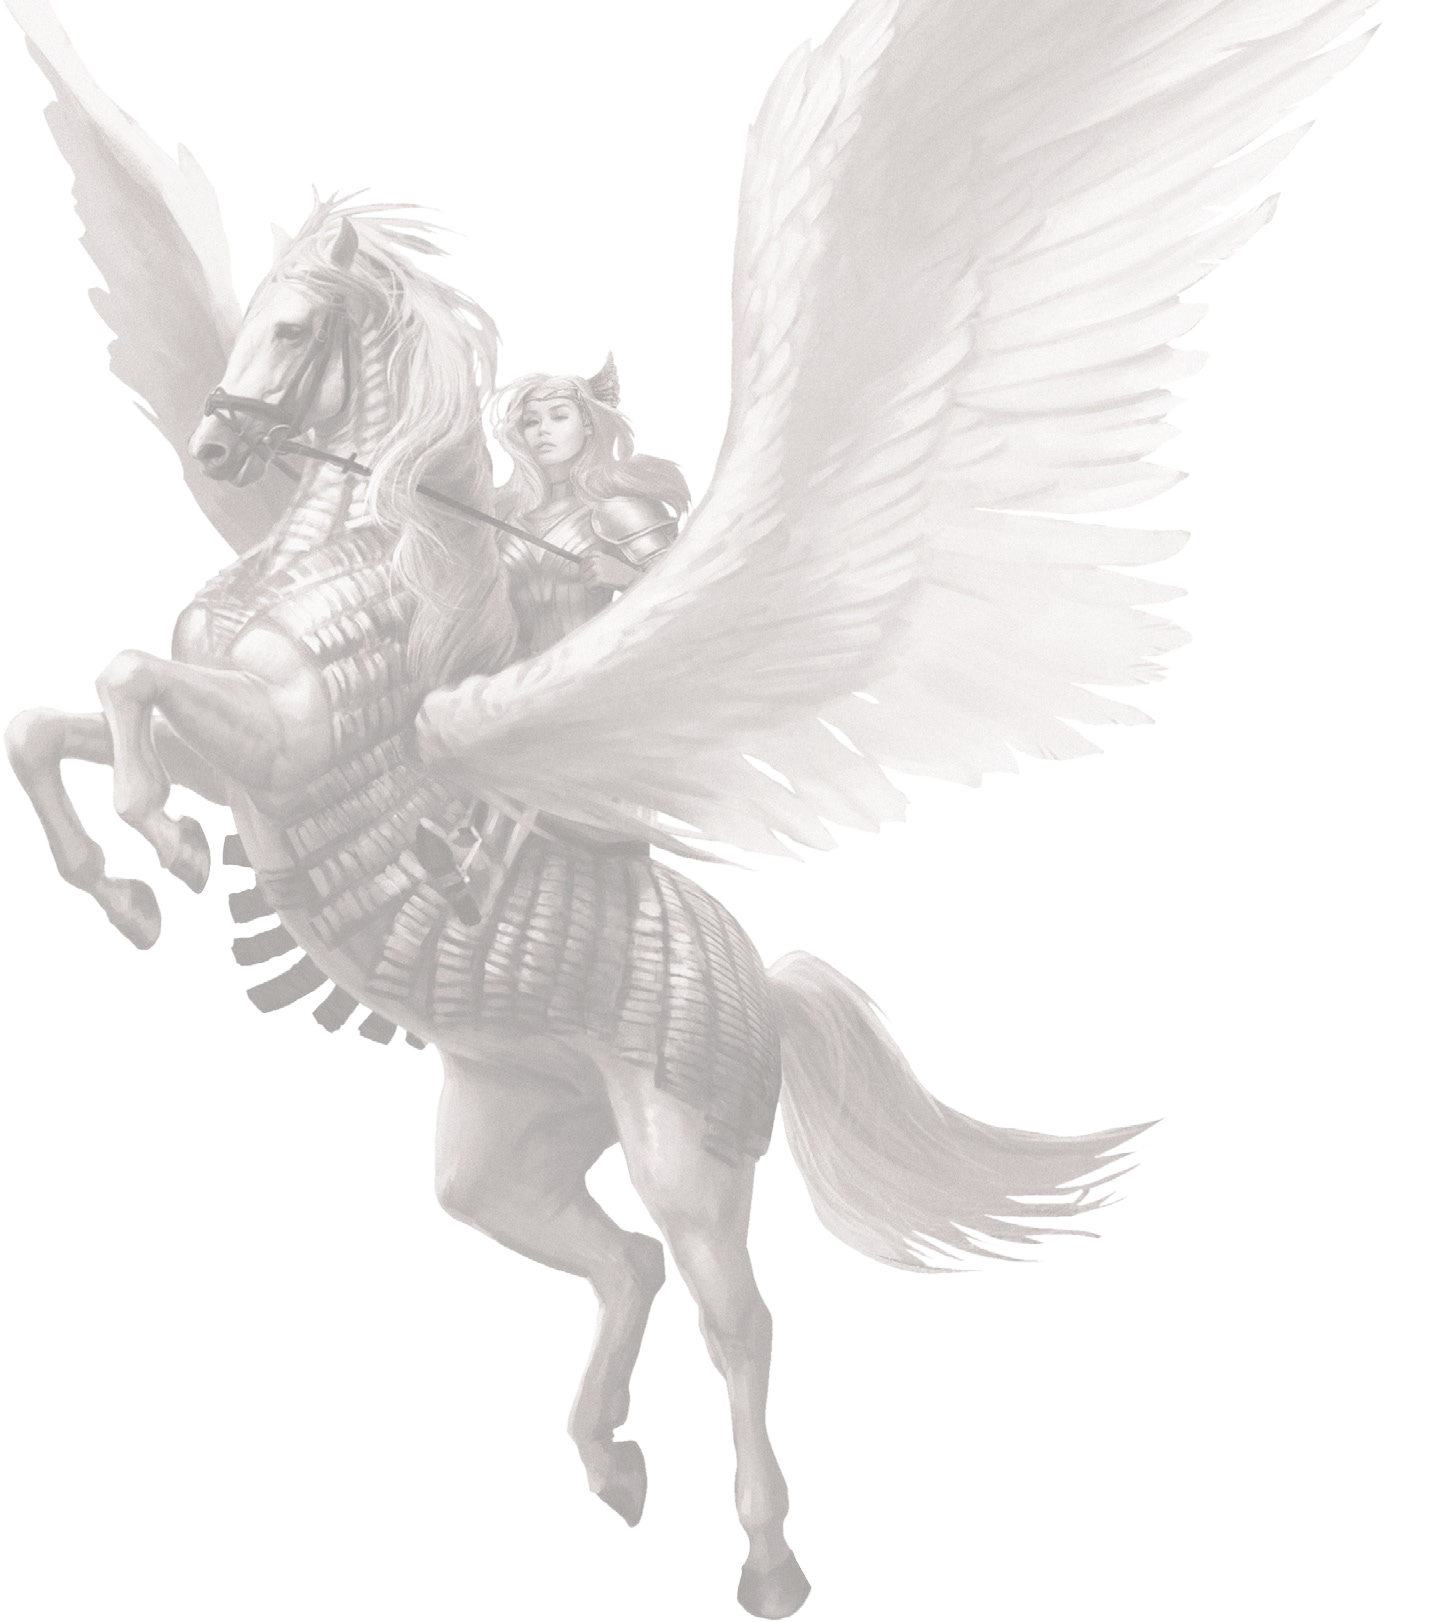
\includegraphics[width=0.5\linewidth]{\art/pegasi.png}};
\end{tikzpicture}

\subsection*{Other Fields}

\begin{figure}[H]
  \begin{minipage}[t]{0.47\textwidth}
    \vspace{0pt}
    \centering
    \textbf{Tree of Knowledge}\par
    \framedimage[\linewidth]{\map_locations/tree_of_knowledge.jpg}
    \caption{\small Category: \textbf{Visitable}\\You may
      \includesvg[height=8px]{\svgs/pay_v2.svg}
       3 \includesvg[height=8px]{\svgs/valuablegreater.svg} or
       10 \includesvg[height=8px]{\svgs/gold.svg} to gain
       2 \includesvg[height=8px]{\svgs/exp.svg}.}
  \end{minipage}\hfill
  \begin{minipage}[t]{0.47\textwidth}
    \vspace{0pt}
    \centering
    \textbf{Redwood Observatory}\par
    \framedimage[\linewidth]{\map_locations/redwood_observatory.jpg}
    \caption{\small Category: \textbf{Visitable}\\Discover a face down Tile adjacent to this one.}
  \end{minipage}
\end{figure}

\begin{figure}[H]
  \begin{minipage}[t]{0.47\textwidth}
    \vspace{0pt}
    \centering
    \phantom{j}\textbf{Grail}\par
    \framedimage[\linewidth]{\map_locations/grail.jpg}
    \caption{\small Category: \textbf{Visitable}\\Gain a Grail Token.
    Only one Grail Token can exist in the game, do not gain another if this Field's Black Cube is removed or if there are multiple Grail Fields.
    The Token's effects are described in the Scenario's description.
    \phantom{\ldots\ldots\ldots}}
  \end{minipage}\hfill
  \begin{minipage}[t]{0.47\textwidth}
    \vspace{0pt}
    \centering
    \phantom{j}\textbf{Market of Time}\par
    \framedimage[\linewidth]{\map_locations/market_of_time.jpg}
    \caption{\small Category: \textbf{Visitable}\\ Remove one card from your hand.
      Then \textbf{Search (2)} the Ability, Spell, or Artifact Deck.
    }
  \end{minipage}
\end{figure}

\begin{figure}[H]
  \begin{minipage}[t]{0.47\textwidth}
    \vspace{0pt}
    \centering
    \phantom{j}\textbf{Hill Fort}\par
    \framedimage[\linewidth]{\map_locations/hill_fort.jpg}
    \caption{\small Category: \textbf{Visitable}\\
      You may immediately Reinforce one of your \includesvg[height=8px]{\svgs/bronze.svg} or \includesvg[height=8px]{\svgs/silver.svg} Units.
      The Reinforcement cost is reduced by 3 \includesvg[height=8px]{\svgs/gold.svg} to a minimum of 0.}
  \end{minipage}\hfill
  \begin{minipage}[t]{0.47\textwidth}
    \vspace{0pt}
    \centering
    \phantom{j}\textbf{Prison}\par
    \framedimage[\linewidth]{\map_locations/prison.jpg}
    \caption{\small Category: \textbf{Visitable}\\
      Gain a Secondary Hero.
      Place their model on this Field.
      If you already have a Secondary Hero, gain 3 \includesvg[height=8px]{\svgs/gold.svg} instead.}
  \end{minipage}
\end{figure}

\begin{figure}[H]
  \begin{minipage}[t]{0.47\textwidth}
    \vspace{0pt}
    \centering
    \textbf{Magic Spring}\par
    \framedimage[\linewidth]{\map_locations/magic_spring.jpg}
    \caption{\small Category: \textbf{Visitable}\\
      You may look at the top 3 Cards of your Discard Pile and return one of them to your Hand.
      Return the remaining cards to the top of your Discard Pile in any order.}
  \end{minipage}\hfill
  \begin{minipage}[t]{0.47\textwidth}
    \vspace{0pt}
    \centering
    \phantom{j}\textbf{Witch Hut}\par
    \framedimage[\linewidth]{\map_locations/witch_hut.jpg}
    \caption{\small Category: \textbf{Visitable}\\
      \textbf{Choose one}: Remove an Ability card from your hand OR look at the top card of the Ability Deck and put that card into your hand or into the Ability Deck Discard Pile.}
  \end{minipage}
\end{figure}

\begin{figure}[H]
  \begin{minipage}[t]{0.47\textwidth}
    \vspace{0pt}
    \centering
    \phantom{j}\textbf{Obelisk}\par
    \framedimage[\linewidth]{\map_locations/obelisk.jpg}
    \caption{\small Category: \textbf{Flaggable}\\
      The Obelisk's effects depend on the Scenario.
      When you Flag this Field, do not remove any enemy Faction Cubes; multiple players may have a Faction Cube on this Field.}
  \end{minipage}\hfill
    \begin{minipage}[t]{0.47\textwidth}
    \vspace{0pt}
    \captionsetup{singlelinecheck=off}
    \centering
    \phantom{j}\textbf{Scholar}\par
    \framedimage[\linewidth]{\map_locations/scholar.jpg}
    \caption[scholar they]{\small Category: \textbf{Visitable}\\
      Roll 1 Attack Die.
      Depending on the result, do the following:
      \begin{itemize}
        \setlength\itemsep{-0.2em}
        \item[ \textbf{+1}] - Gain a Statistic Card of your choice or Remove a Statistic Card from your hand.
        \item[\textbf{0}] - Draw 2 Cards from the Ability Deck, gain one of them and discard the other.
        \item[\textbf{-1}] - Draw 2 Cards from the Spell Deck, gain one of them and discard the other.
        \end{itemize}
       }
  \end{minipage}
\end{figure}

\begin{figure}[H]
  \begin{minipage}[t]{0.47\textwidth}
    \vspace{0pt}
    \centering
    \textbf{Dragon Utopia}\par
    \framedimage[\linewidth]{\map_locations/dragon_utopia.jpg}
    \caption{\small Category: \textbf{Flaggable}\\Effects depend on the Scenario.}
  \end{minipage}\hfill
  \begin{minipage}[t]{0.47\textwidth}
    \vspace{0pt}
    \centering
    \textbf{University}\par
    \framedimage[\linewidth]{\map_locations/university.jpg}
    \caption{\small Category: \textbf{Visitable}\\
      \includesvg[height=8px]{\svgs/pay_v2.svg} 6 \includesvg[height=8px]{\svgs/gold.svg} to \textbf{Search (4)} the Ability Discard Pile.}
  \end{minipage}
\end{figure}

\begin{multicols*}{2}

{\centering\phantom{Star Axis}\par}
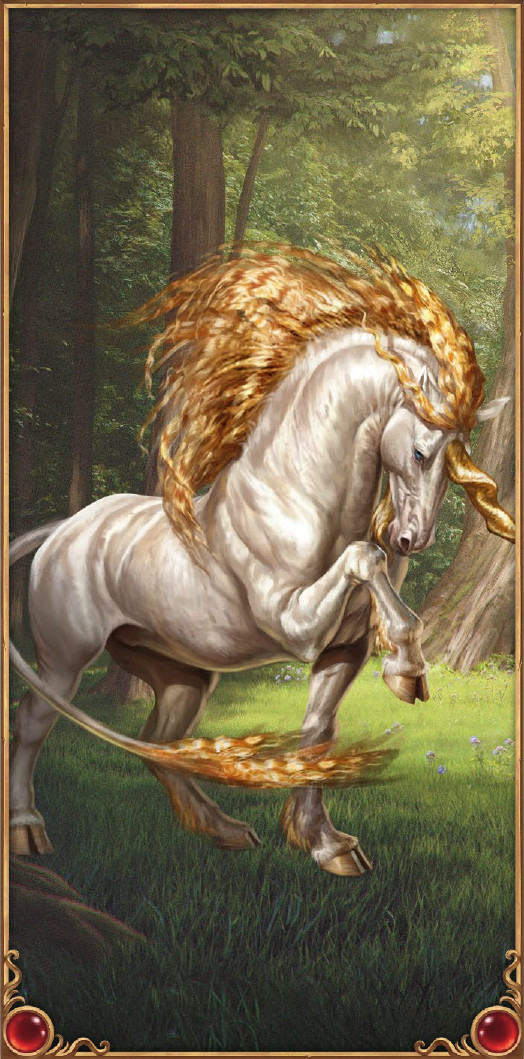
\includegraphics[width=\linewidth]{\art/unicorn.jpg}

\columnbreak

{\centering\textbf{Star Axis}\par}
\framedimage[\linewidth]{\map_locations/star_axis.jpg}
{\small Category: \textbf{Flaggable}\\
  You may Remove one of your Statistic cards from your hand and replace it with an \textbf{Empowered} one of the same type.
  When you Flag this Field, do not remove any enemy Faction Cubes; multiple players may have a Faction Cube on this Field.
}

\bigskip

{\centering\textbf{\hypertarget{Random Town}{Random Town}}\par}
\framedimage[\linewidth]{\map_locations/random_town.jpg}
{\small Category: \textbf{Flaggable}\\
  When revealed, all players roll 2 \includesvg[height=10px]{\svgs/resource_die.svg}.
  The highest roller chooses an unused Faction.
  The random Town is defended by Units from that Faction.
  They have a "Pack" of \includesvg[height=10px]{\svgs/bronze.svg}, two "Packs" of \includesvg[height=10px]{\svgs/silver.svg}, and two "Fews" of \includesvg[height=10px]{\svgs/golden.svg} Units.
  The \includesvg[height=10px]{\svgs/bronze.svg} Unit is chosen by the player who controls the Units during that Combat.
  Flagging it increases \includesvg[height=10px]{\svgs/gold.svg} production by 10, which is also gained immediately if you are the first to Flag it.
}

\end{multicols*}
